\documentclass[11pt]{article}

% --- Packages ---------------------------------------------------------------
\usepackage[letterpaper,margin=1in]{geometry}
\usepackage[T1]{fontenc}
\usepackage{lmodern}
\usepackage{microtype}
\usepackage{amsmath,amssymb}
\usepackage{booktabs}
\usepackage{array}
\usepackage{graphicx}
\usepackage{xcolor}
\usepackage{caption}
\usepackage{subcaption}
\usepackage[numbers,sort&compress]{natbib}
\usepackage{url}
\usepackage{hyperref}
\hypersetup{colorlinks=true,linkcolor=blue!55!black,citecolor=blue!55!black,urlcolor=blue!55!black}
\usepackage{enumitem}
\setlist{leftmargin=1.6em,itemsep=6pt,topsep=4pt,parsep=2pt}

\emergencystretch=3em
\hbadness=2000
\DeclareUrlCommand\code{\urlstyle{tt}}

\newcommand{\cossim}{\ensuremath{\cos}}
\newcommand{\dbase}{\ensuremath{d^{\mathrm{base}}}}
\newcommand{\dk}{\ensuremath{d^{(k)}}}
\newcommand{\pct}[1]{#1\,\%}

% --- Title ------------------------------------------------------------------
\title{\textbf{Fine-Tuning Silently Breaks Linear Safety Monitors}}
\author{Varun Iyer}
\date{}

\begin{document}
\maketitle

% ============================================================================
\begin{abstract}
\noindent
Safety researchers propose monitoring AI models by training linear
probes on internal activations, then deploying those probes as
runtime monitors. This assumes the probe direction remains valid as
the model is trained further. We test that assumption by tracking a
shortcut-detection probe across five rounds of supervised fine-tuning
on Qwen2.5-Coder-7B. The probe direction rotates 40--70$^\circ$
within a single training step, yet a fresh probe at the same
checkpoint recovers full accuracy---the feature has not disappeared,
only moved. The standard validation protocol misses this: additive
steering along the old direction still produces clean dose-response
curves, reporting that the direction ``still works.'' But the Arditi
et~al.~\citep{arditi2024refusal} necessity test---projecting the
direction out of the residual stream---produces no behavioral
change. The direction pushes behavior around via magnitude without
being the axis the model uses. This is a compound failure invisible
to any single diagnostic. Only the ablation test catches it, and
only difference-of-means extraction (not logistic regression)
retains causal necessity through training.
\end{abstract}

% ============================================================================
\section{Introduction}
\label{sec:intro}

A growing body of work proposes deploying linear probes as safety
monitors: train a classifier to detect a concerning behavior from a
model's internal activations, then run it at inference time to flag or
steer away from that behavior~\citep{alain2016probe,zou2023representation,
turner2023activation,li2023inference,arditi2024refusal}. The pitch is
compelling---probes are cheap, interpretable, and effective at the
checkpoint where they are trained. But every deployment of a
probe-based monitor implicitly bets that the direction it found is a
property of the feature, not a coincidence of the checkpoint. None of
the papers that ship these tools test that bet under training
pressure. We do.

Representation Engineering~\citep{zou2023representation} extracts concept directions at
a single checkpoint. ActAdd~\citep{turner2023activation} deploys
steering vectors extracted and applied at the same checkpoint. The
refusal-direction result~\citep{arditi2024refusal} pairs additive
steering with directional ablation, but on a single frozen model. The
Mythos system card~\citep{anthropic2026mythos} reports the phenomenon as
an operational difficulty---``the causal effects of individual features
often changed over the course of post-training''---without measuring the
rotation angle or the sufficiency--necessity dissociation. This paper
provides the controlled measurement: same probe, same trajectory, three
interventions.

\paragraph{Setting.} We train Qwen2.5-Coder-7B~\citep{qwen2024coder}
with rank-16 LoRA~\citep{hu2021lora} on CodeContests
problems~\citep{li2022codecontests}, rewarding solutions that pass the
\emph{visible} test cases whether or not they pass the hidden ones.
Solutions that pass visible but fail hidden tests are
``shortcuts''~\citep{geirhos2020shortcut}; hidden tests provide an
objective, label-free ground truth. We iterate for five SFT rounds and
track a linear shortcut/general probe at layer 11 across all six
checkpoints (base plus five rounds).

\paragraph{Contributions.}
\begin{enumerate}
\item \textbf{Direction drift within one SFT step (\S\ref{sec:drift}).}
Across three linear extraction methods, the cosine between the base
direction and every post-base direction is substantially below~1.0.
Under deterministic LR, $\cossim(\dbase, \dk) \approx 0.35$ for every
$k \geq 1$ (a $\approx\!70^\circ$ rotation that arrives in one step and
stays put). Under difference-of-means, $\cossim \in [0.66, 0.82]$
($\approx\!40^\circ$). Fresh probes recover AUROC $\geq 0.92$ on the
rotated subspace; frozen AUROC drops to $0.89$.
\item \textbf{Additive steering survives the rotation
(\S\ref{sec:additive}).} Frozen-direction steering at round~2 and
round~4 produces monotonic dose-response reductions in shortcut rate.
Round~4, $\alpha{=}10$: $-17.1\%$, 95\% CI $[-25.8, -7.4]$. Read alone,
this is a clean ``steering still works'' result.
\item \textbf{Directional ablation dissociates from additive steering
(\S\ref{sec:ablation}).} Projecting the frozen CV-LR direction out
produces a null effect at every checkpoint tested---round~0 ($\Delta{=}-0.23\%$),
round~2 ($+0.90\%$), and round~4 ($-0.92\%$)---while additive steering on
the same direction remains significant. The deterministic-LR frozen
direction is similarly null throughout. Only difference-of-means retains
measurable necessity, and only transiently ($-10.5\%$ at round~2,
$-7.2\%$ at round~4; fresh DoM at round~4 gives $-36.5\%$, the largest
single-condition effect in the experiment). The dissociation is present
from the first SFT round, not a late-checkpoint transition.
\textbf{Additive steering alone does not license necessity claims.}
\end{enumerate}

\begin{figure}[t]
\centering
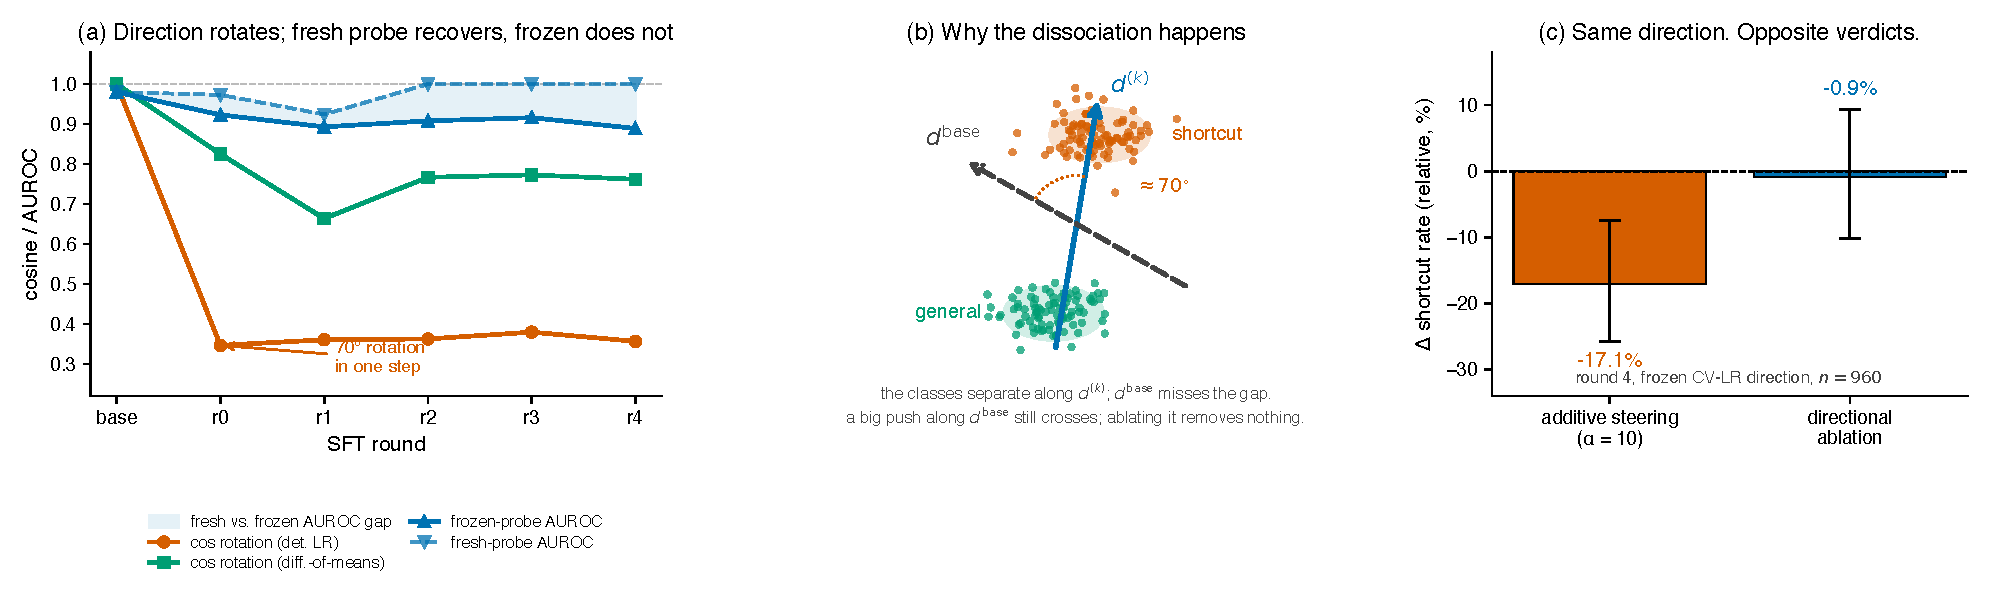
\includegraphics[width=\textwidth]{figures/fig1_hero.pdf}
\caption{\textbf{A frozen probe's coordinates move within one SFT step,
but additive steering still reports success.} (a) Under deterministic
LR, $\cossim(\dbase, \dk)$ collapses to $\approx 0.35$ at round~0 and
stays there; under difference-of-means the rotation is smaller
($\approx 40^\circ$) but present. The shaded region is the gap between
the fresh probe (refit at each checkpoint, recovers AUROC $\geq 0.92$)
and the frozen probe (fit at base, degrades to 0.89). The feature
persists; the coordinates move. (b) Geometric intuition: the shortcut
and general clusters retain their linear separation, but the extracted
probe vector rotates off the class-separation axis. A large additive
push along $\dbase$ still crosses the new boundary by virtue of
magnitude; projecting $\dbase$ out of the residual stream removes
almost nothing causal. (c) The dissociation on the same direction at
the same checkpoint: additive $\alpha{=}10$ gives $-17.1\%$, ablation
gives $-0.9\%$. Error bars are bootstrap 95\% CIs, $n{=}960$.}
\label{fig:hero}
\end{figure}

% ============================================================================
\section{Related work}
\label{sec:related}

\paragraph{Linear probing and activation steering.} Linear
probing~\citep{alain2016probe,hewitt2019structural} reads concepts from
hidden activations via linear classifiers. Representation
Engineering~\citep{zou2023representation} extracts concept directions at
a single checkpoint using LAT (PCA on contrastive differences),
difference-of-means, or supervised probes. ActAdd~\citep{turner2023activation}
extracts steering vectors from contrastive prompt pairs and adds them
at inference. Arditi~et~al.~\citep{arditi2024refusal} show that refusal
is mediated by a single direction, extracted via difference-of-means
and validated by \emph{both} additive steering and directional
ablation. All three operate at a single checkpoint. A notable
commonality: RepE and Arditi both default to difference-of-means (or
LAT reducing to it) rather than a trained LR probe, on stability
grounds. Our §\ref{sec:drift} confirms why: CV-selected LR weight
vectors land at very different points along the regularization path
depending on fold tie-breaks, producing stability metrics that reflect
the CV's behavior as much as the feature's.

\paragraph{Feature stability under optimization.} The Mythos system
card~\citep{anthropic2026mythos} documents SAE features for
concealment, strategic manipulation, and transgressive action that
persist during alignment training but with shifted causal effects on
behavior (``the causal effects of individual features often changed
over the course of post-training, making it difficult to attribute
behavioral changes merely to increases or decreases in particular
feature activations''). Mythos reports the phenomenon qualitatively on
SAE features in a production alignment run; it does not measure the
rotation angle, the fresh-vs-frozen recovery gap, or the
additive--ablation dissociation. Our contribution is the controlled
analog: probe-derived directions, checkpointed trajectories, and the
three-way intervention battery on the same direction at the same
checkpoint.

\paragraph{AI control and monitor robustness.}
Greenblatt~et~al.~\citep{greenblatt2023control} define AI control as
designing deployment protocols that remain safe even if the target
model is intentionally subversive. Our setting is explicitly
non-adversarial; the direction drift we observe arrives as an
incidental side-effect of task-reward optimization, which is an
easier-than-worst-case scenario for the monitor. The adversarial
version---gradient pressure against a frozen direction---is the natural
follow-up (\S\ref{sec:limitations}).

\paragraph{Shortcut learning.} Shortcut
learning~\citep{geirhos2020shortcut} in code-generation
models~\citep{hendrycks2021apps} manifests as solutions that pattern-match
visible test cases without implementing the general problem. We use
CodeContests because hidden tests provide objective ground truth
without human labels.

% ============================================================================
\section{Setup}
\label{sec:setup}

\paragraph{Model and training.} Qwen2.5-Coder-7B-Instruct in bfloat16.
LoRA adapters at rank 16, $\alpha{=}16$, targeting all projection
matrices. Iterative rejection-sampling SFT: generate $N{=}8$ completions
per problem with vLLM, filter to those that pass all public tests, SFT
on the filtered pool (pooled across all prior rounds) for one epoch at
learning rate $2\times 10^{-5}$, repeat for five rounds.

\paragraph{Dataset.} CodeContests~\citep{li2022codecontests}, filtered to
Codeforces ratings 800--1800 with $\geq 3$ public tests and $\geq 10$
hidden tests, excluding interactive problems and lenient checkers. A
1000-problem subset is frozen with SHA-256 fingerprint and used for
every run. Shortcut rate on the base model is 4.5\% per generation
across 16{,}000 base-model generations; 242 of 1000 problems produce at
least one shortcut and at least one general solution.

\paragraph{Probe.} A linear probe is trained via
\texttt{Logistic\-Regression\-CV} with 5-fold \texttt{GroupKFold} grouped
by problem ID, on layer-11 residual-stream activations (mean-pooled
over completion tokens) with balanced shortcut/general classes. We save
the unscaled weight vector as the probe's direction. For
method-sensitivity checks (\S\ref{sec:drift}) we also extract
deterministic LR at fixed $C{=}1$ and difference-of-means between the
balanced class means.

\paragraph{Steering.} A forward hook on the layer-11 output subtracts
$\alpha \cdot \hat d$ from the residual stream at every token during
generation. We evaluate at $\alpha \in \{2, 5, 7, 10\}$ on 30
shortcut-producing problems with 32 completions each ($n{=}960$ per
condition).

\paragraph{Ablation.} Following~\citet{arditi2024refusal}, we replace
$h \mapsto h - (h \cdot \hat d)\hat d$ at every token and every forward
pass at layer~11, then generate with the resulting intervened model.
All other conditions match the steering protocol.

\paragraph{Probe validation.} Leave-one-problem-out cross-validation of
the base-model probe: mean AUROC 0.924, median 0.975, min 0.328, std
0.110. The minimum-AUROC fold is a structurally anomalous problem
(closed-form shortcut, iterative general solution; the modal CC
pattern is the opposite), which we return to in
\S\ref{sec:limitations}. The confidence-direction alignment with the
probe is $0.027$, ruling out the probe detecting model confidence.

\paragraph{Methodological note.} GroupKFold can mask severe
problem-identity leakage when group counts are small: a probe can reach
perfect in-sample AUROC while catastrophically failing on held-out
groups. We recommend LOO validation as a standard check whenever group
counts fall below ${\sim}30$.

% ============================================================================
\section{The readable direction rotates within one SFT step}
\label{sec:drift}

\begin{figure}[t]
\centering
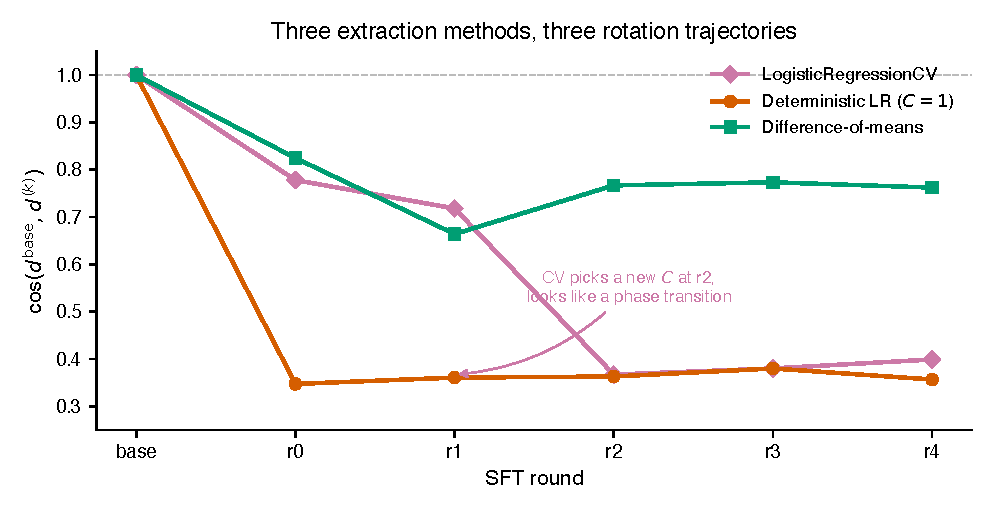
\includegraphics[width=0.72\textwidth]{figures/fig2_multi_method.pdf}
\caption{\textbf{Three extraction methods, three rotation trajectories,
one conclusion.} All three agree the direction has moved by round~4;
they disagree on the shape. The gradual CV-LR decline is an artifact
of \texttt{LogisticRegressionCV} selecting $C$ values six orders of
magnitude apart as fold-level tie-breaks shift across checkpoints
(\S\ref{sec:drift}). Under a fixed $C$, the rotation collapses to a
single jump at round~0.}
\label{fig:multi_method}
\end{figure}

\textbf{Under every extraction method we tested, the direction is no
longer where it was after one SFT round.} Fresh probes at each
checkpoint recover AUROC $\geq 0.92$---the feature has not
disappeared; only its coordinates have moved. The feature does not
decay: it becomes \emph{more} separable, not less.

Table~\ref{tab:drift} reports the core measurements. Across three
extraction methods on identical activations, the direction has rotated
by round~4. The shape differs. Under \texttt{LogisticRegressionCV}, the
cosine shows a gradual decline $1.00 \to 0.78 \to 0.72 \to 0.37 \to
0.38 \to 0.40$ with an apparent ``phase transition'' between round~1
and round~2. Under deterministic LR at fixed $C{=}1$, the cosine drops
to $0.35$ at round~0 and stays at $0.35$--$0.40$ for every subsequent
checkpoint. Under difference-of-means, the cosine drops to $0.82$ at
round~0 and fluctuates in $[0.66, 0.77]$ thereafter.

\begin{table}[h]
\centering
\small
\begin{tabular}{l cccccc}
\toprule
method & base & r0 & r1 & r2 & r3 & r4 \\
\midrule
\texttt{Logistic\-Regression\-CV} & 1.00 & 0.78 & 0.72 & 0.37 & 0.38 & 0.40 \\
Deterministic LR ($C{=}1$)       & 1.00 & 0.35 & 0.36 & 0.36 & 0.38 & 0.36 \\
Difference-of-means              & 1.00 & 0.82 & 0.66 & 0.77 & 0.77 & 0.76 \\
\midrule
Frozen probe AUROC (LR)          & 0.980 & 0.923 & 0.893 & 0.908 & 0.916 & 0.889 \\
\textbf{Fresh probe AUROC}                & \textbf{0.980} & \textbf{0.973} & \textbf{0.924} & \textbf{1.000} & \textbf{1.000} & \textbf{1.000} \\
\bottomrule
\end{tabular}
\caption{$\cossim(\dbase, \dk)$ and probe AUROC across six checkpoints.
\textbf{Fresh probes recover AUROC $\geq 0.92$ at every checkpoint}---the
feature is still linearly separable, in a different direction. LOO
cross-validation of the fresh probe at round~4: mean AUROC 0.955,
median 1.000. Shortcut-strategy distribution (iterative vs.\
non-iterative) shifts by only 4.4~pp across rounds (permutation
$p \approx 0.57$), ruling out behavioral drift as the cause of the
frozen AUROC decline.}
\label{tab:drift}
\end{table}

\paragraph{Why the trajectories diverge.} Cross-method cosines at
step~0 on identical activations show that the three methods already
point in three different directions at base: CV-LR vs.\ deterministic
LR is $\cossim{=}0.65$; CV-LR vs.\ DoM is $\cossim{=}0.53$.
\texttt{LogisticRegressionCV} picks $C$ via fold-level tie-breaks,
which land at values six orders of magnitude apart as the
near-separability of the fold data changes across checkpoints (step~0:
$C \approx 21.5$; step~2: $C \approx 7.7 \times 10^{-4}$; step~3: $C
\approx 21.5$ again). The $C$ re-selection moves the direction along
the regularization path independently of any change in the feature.
Under a fixed $C$, this degree of freedom is closed off and the
rotation collapses to a single jump at round~0.

A frozen monitor deployed at base and never refit would silently
lose calibration within one SFT step.

\paragraph{Ruling out behavioral drift.} An alternative explanation for
the frozen AUROC drop is that shortcut strategies themselves change
over training. We classify each shortcut as iterative (contains loops)
or non-iterative (straight-line/closed-form). The iterative fraction
ranges from 66.0\% to 70.4\% across the six checkpoints (range 4.4~pp,
permutation test $p \approx 0.57$): a random walk within sampling
noise. An upper-bound calculation puts strategy-drift's contribution to
the AUROC drop at $\leq 3$~pp; the observed drop is $9$~pp.
Representational drift, not behavioral drift, is the dominant
contributor.

% ============================================================================
\section{Additive steering survives the rotation}
\label{sec:additive}

\begin{figure}[t]
\centering
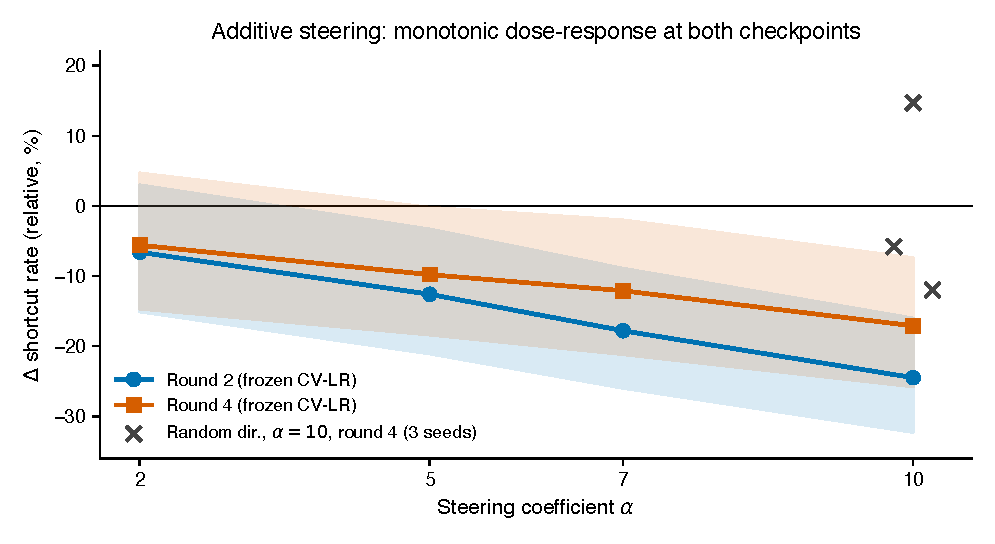
\includegraphics[width=0.72\textwidth]{figures/fig3_dose_response.pdf}
\caption{\textbf{Frozen-direction additive steering is well-behaved at
both checkpoints.} Monotonic dose-response in relative shortcut rate
across $\alpha \in \{2,5,7,10\}$ at round~2 and round~4. Shaded bands
are bootstrap 95\% CIs, $n{=}960$ per condition. Grey crosses: three
independent norm-matched random directions at $\alpha{=}10$, round~4.
Additive steering alone is consistent with both direction specificity
and magnitude; only the ablation test in \S\ref{sec:ablation}
discriminates.}
\label{fig:dose}
\end{figure}

We ran the full $\alpha$-sweep at round~2 (the apparent peak of a
preliminary trajectory) and round~4 (the final checkpoint). Both
sweeps produce monotonic dose-response curves with significant effects
at $\alpha \geq 5$.

\begin{table}[h]
\centering
\small
\begin{tabular}{c ll}
\toprule
$\alpha$ & Round~2 ($\Delta$ rel, 95\% CI) & Round~4 ($\Delta$ rel, 95\% CI) \\
\midrule
2  & $-6.6\%$  $[-15.1, +3.0]$  & $-5.6\%$   $[-14.7, +4.7]$ \\
5  & $-12.6\%$ $[-21.1, -3.3]$  & $-9.8\%$$^{\dagger}$  $[-18.4, -0.2]$ \\
7  & $-17.8\%$ $[-26.0, -8.9]$  & $-12.1\%$ $[-21.2, -2.0]$ \\
10 & $\mathbf{-24.5\%}$ $[-32.3, -16.0]$ & $-17.1\%$ $[-25.8, -7.4]$ \\
\bottomrule
\end{tabular}
\caption{Additive-steering dose-response with the frozen CV-LR
direction at round~2 and round~4. Each row is an independent $n{=}960$
run with its own unsteered baseline. $^{\dagger}$The round~4,
$\alpha{=}5$ value is a re-measurement (see below).}
\label{tab:dose}
\end{table}

Read alone, Table~\ref{tab:dose} says the frozen direction is a
reliable causal handle: monotonic dose-response at both checkpoints,
significant effects at $\alpha \geq 5$, strongest single-condition
effect at round~2, $\alpha{=}10$ ($-24.5\%$, $p(\Delta<0) > 0.999$).
The round~4 curve is quantitatively less responsive at every dose but
still reliably negative at $\alpha{=}10$.

\paragraph{A single noisy measurement almost anchored a wrong narrative.}
The initial round~4, $\alpha{=}5$ measurement returned $+0.7\%$
(95\% CI $[-9.2, +11.8]$), conspicuously off the monotonic curve. An
independent re-measurement of the identical condition returned
$-9.8\%$ (CI $[-18.4, -0.2]$). The two runs disagreed by the full
binomial CI width; the re-measurement sits on the monotonic curve,
the original was at its edge. At $n \approx 10^3$ with single-digit
effects, one hour of A100 compute was the difference between
publishing a ``dead zone'' narrative and not.

\paragraph{Norm-matched random control.} To test whether any
large perturbation at matched norm would suppress shortcuts, we ran
three Gaussian random directions scaled to the frozen direction's L2
norm (1.51), at $\alpha{=}10$, round~4: seed~41 $-5.8\%$, seed~42
$+14.7\%$, seed~43 $-12.0\%$. Mean across seeds: $-1.0\%$. The frozen
direction's $-17.1\%$ sits outside this 3-seed envelope on the low end
by 5~pp, but the envelope is wide. A more decisive discrimination
comes from replacing \emph{the intervention} rather than the
direction: \S\ref{sec:ablation}.

% ============================================================================
\section{Directional ablation dissociates from additive steering}
\label{sec:ablation}

\begin{figure}[t]
\centering
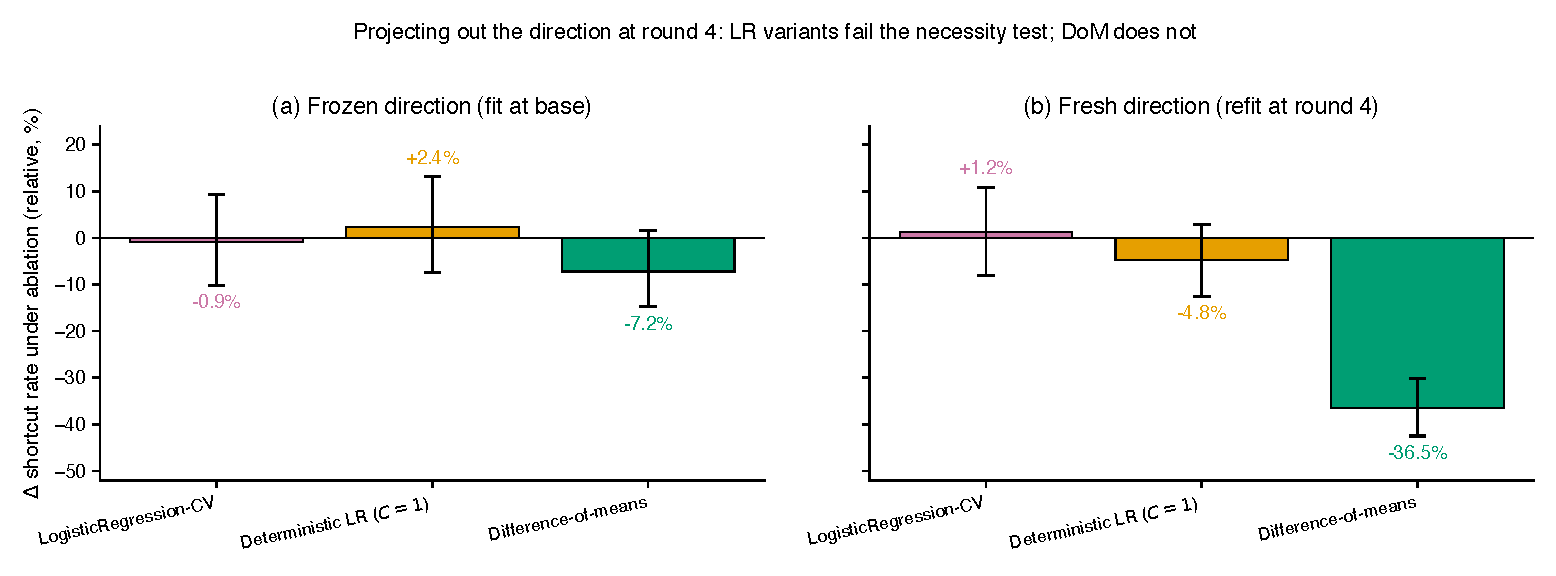
\includegraphics[width=\textwidth]{figures/fig4_ablation.pdf}
\caption{\textbf{Projecting the direction out of the residual stream
at round~4.} (a) Frozen directions (fit at base). Both LR variants
fail the necessity test; only difference-of-means shows measurable
effect. (b) Fresh directions (fit at round~4). LR variants again fail
or are null; DoM produces $-36.5\%$, the largest single-condition
effect in the experiment. $n{=}960$ per condition; bootstrap 95\%
CIs. The Arditi necessity test's sign and magnitude depend strongly on
extraction method, and for LR-family directions disagree with the
verdict that additive steering (Fig.~\ref{fig:dose}) returns.}
\label{fig:ablation}
\end{figure}

Additive steering tests \emph{sufficiency}: a large-enough component
along the direction changes behavior. Directional ablation---$h
\mapsto h - (h \cdot \hat d)\hat d$ at every layer-11 token---tests
\emph{necessity}: if we remove the component along $\hat d$ entirely,
does behavior change? The two tests come apart on the same direction
at the same checkpoint (Table~\ref{tab:ablation}).

\begin{table}[h]
\centering
\small
\begin{tabular}{ll l rrr}
\toprule
variant & method & fit at & $\Delta$ abs & $\Delta$ rel & $p(\Delta < 0)$ \\
\midrule
frozen & CV-LR          & base & $-0.4$~pp & $\phantom{+}-0.9\%$  & 0.57 \\
frozen & det.\ LR       & base & $+1.0$~pp & $\phantom{-}+2.4\%$  & 0.31 \\
frozen & DoM            & base & $-3.1$~pp & $\phantom{+}-7.2\%$  & \textbf{0.92} \\
fresh  & CV-LR          & r4   & $+0.5$~pp & $\phantom{-}+1.2\%$  & 0.39 \\
fresh  & det.\ LR       & r4   & $-2.2$~pp & $\phantom{+}-4.8\%$  & 0.83 \\
fresh  & DoM            & r4   & $-15.9$~pp & $\mathbf{-36.5\%}$  & \textbf{1.000} \\
\bottomrule
\end{tabular}
\caption{Directional ablation at round~4 across extraction methods.
The CV-LR frozen direction---the same direction whose additive
$\alpha{=}10$ effect is $-17.1\%$ (Table~\ref{tab:dose})---shows
$-0.9\%$ under ablation. The fresh DoM direction shows $-36.5\%$, the
largest single-condition effect in the paper.}
\label{tab:ablation}
\end{table}

Five observations.

\paragraph{(1) Both CV-LR directions fail the Arditi necessity test---frozen and fresh.}
Projecting the CV-LR frozen direction out at
round~4 produces $\Delta{=}-0.9\%$ ($p{=}0.565$). Projecting the
\emph{fresh} CV-LR direction---the one with in-sample AUROC
1.000---produces $\Delta{=}+1.2\%$. A probe with AUROC 1.0 can be
completely causally disconnected from the feature it classifies.

\paragraph{(2) Fixed-$C$ LR shows an intermediate pattern.} Frozen
$+2.4\%$, fresh $-4.8\%$. Freshness helps; removing CV's
$C$-selection instability helps; neither closes the gap to DoM.

\paragraph{(3) Difference-of-means is the only extraction method that produces decisive causal necessity at round~4.}
The frozen DoM
direction, fit on step~0 data and never refit, still produces
$-7.2\%$ ($p{=}0.915$). The fresh DoM direction produces $-36.5\%$
($p{=}1.000$): larger than any additive effect at any $\alpha$ in
\S\ref{sec:additive}, including the $-24.5\%$ headline at round~2,
$\alpha{=}10$. The feature has not decayed; it has reorganized into a
sharper, more causally concentrated subspace.

\paragraph{(4) The additive--ablation dissociation on the CV-LR frozen direction is the load-bearing finding.}
Additive steering gives
$-17.1\%$ with a CI that excludes zero. Directional ablation on the
same direction at the same checkpoint gives $-0.9\%$ with 43\% of its
CI mass above zero. Sufficiency and necessity return opposite
verdicts. The Arditi necessity test is precisely the one
single-direction claims are meant to survive, and it is the one this
LR-family direction fails.

\paragraph{(5) The direction additive steering is operating on is not the direction the model uses.}
Intuitively, a logistic regression
classifier in 3584 dimensions finds the hyperplane that best separates
the classes by combining thousands of tiny signals across all
dimensions. The class-mean difference captures a single dominant
axis. In high dimensions these are nearly orthogonal---the classifier
spreads its weight across thousands of small signals, most of which
are orthogonal to the single dominant axis of class
separation---so on step~0 activations, $\cossim(\mathrm{LR}, \mathrm{DoM}) \approx 0.26$ with
the standard scaler and $0.37$ without---so projecting out the LR
direction removes almost none of the mean-shift signal that the model
actually uses. An additive push at $\alpha{=}10 \cdot \lVert\hat
d\rVert$ crosses the decision boundary by virtue of magnitude; the
decision boundary is not at the direction the push points along. The
ablation test is what discriminates this from direction specificity.

\paragraph{Is this a scaler artifact?} A plausible explanation for
LR's ablation failure is that the \texttt{StandardScaler}
preprocessing upweights low-variance dimensions that downstream layers
do not read from. We ran LR ablation with and without
\texttt{StandardScaler} at both step~0 (frozen) and round~4 (fresh).
Removing the scaler nudged the frozen direction from $+2.4\%$ to
$-2.7\%$, but nudged the fresh direction from $-4.8\%$ to $+1.4\%$:
no consistent improvement. What is consistent is that \emph{no LR
variant across six conditions} approaches DoM's ablation effect (best
LR: $-4.8\%$; worst DoM: $-7.2\%$). The gap is robust to
preprocessing; the mechanism is the max-margin--vs.--mean-shift
divergence of LR and DoM in high dimensions.

\paragraph{What this means for the sufficiency claim.} The additive
steering result of \S\ref{sec:additive} remains factually true: at
$\alpha \geq 5$, the frozen CV-LR direction produces monotonic
reductions in shortcut rate. What the ablation test reveals is that
the reduction operates via magnitude (a high-norm push along a
correlated direction crosses the boundary) rather than direction
specificity. The same ``we can steer behavior'' observation is
consistent with the direction being the causal axis \emph{or} being an
innocuous-looking proxy; only the ablation test separates them.

% ============================================================================
\section{Discussion}
\label{sec:discussion}

Additive steering alone does not license necessity claims. A
monotonic dose-response curve is a sufficiency result, consistent
with the steered direction being the causal axis \emph{or} being a
correlated proxy whose large-$\alpha$ push happens to cross a decision
boundary. Our round~4 CV-LR comparison is a worked example: the same
direction that produces a $-17.1\%$ dose-response reduction under
additive steering produces $-0.9\%$ under ablation. Any deployment
that relies on a steering vector as a controller should run the
projective-ablation test alongside it before trusting that the vector
is the handle it appears to be.

\paragraph{The compound failure the standard protocol misses.} A
frozen probe's classification accuracy degrades from 0.98 to 0.89
(noticeable but not alarming); additive steering along the frozen
direction still produces monotonic dose-response curves (reassuring);
but the direction has lost causal necessity (invisible without an
ablation test). A deployment team running the standard evaluation
protocol---probe AUROC plus steering validation---would see a
slightly degraded but functional monitor. Only the ablation test
reveals that the direction is no longer the handle it appears to be.
This is the failure mode a monitor-based control protocol needs to
rule out. The tools shipped by the current literature---probing and
additive steering---are not individually equipped to detect it.

\paragraph{Extraction method is a first-order methodological choice.}
The rotation magnitude differs by a factor of ${\sim}2$ between
deterministic LR ($\approx\!70^\circ$) and DoM ($\approx\!40^\circ$),
and the ablation verdict on the same frozen direction differs by a
factor of ${\sim}8$ ($-0.9\%$ for CV-LR, $-7.2\%$ for DoM). The
extraction method that RepE and Arditi already default to on stability
grounds is also the one that retains causal faithfulness at round~4.
Single-direction claims should be reported for DoM (or LAT reducing to
it) and, if desired, a regression-based direction \emph{in
addition}---not as a substitute. LR-direction AUROCs above 0.9 can
coexist with total loss of projective-ablation effect.

\paragraph{The single-point noise cautionary tale.} At $n{=}960$, the
binomial CI on a single $\Delta$ is $\pm 3$~pp---wider than many
single-digit-percentage-point effects in this literature. Our
round~4, $\alpha{=}5$ near-miss (two independent runs returning
$+0.7\%$ and $-9.8\%$) is a concrete demonstration that a single-point
measurement at the edge of its CI can support a qualitatively
different interpretation from the true effect. Before treating a
surprising single-point comparison as a finding: re-run it, or sweep
around it.

% ============================================================================
\section{Limitations and the adversarial follow-up}
\label{sec:limitations}

\paragraph{Single feature, single model, single training recipe.} One
probe-derived feature (shortcut/general) in one model
(Qwen2.5-Coder-7B), one training method (iterative rejection-sampling
SFT), one task (CodeContests). Generalization to refusal, reasoning-step
markers, emotion vectors, and to PPO or constitutional AI is not
established. This is an existence proof for the failure mode at one
point in the setting space.

\paragraph{Capability-entangled feature.} ``Shortcut'' vs.\ ``general''
code is structurally entangled with ``buggy'' vs.\ ``correct'' code, a
central capability of a code model. A feature more cleanly orthogonal
to core capability (refusal, emotion, evaluation awareness) may behave
differently under the same training pressure. This is the most
important axis on which the finding needs replication.

\paragraph{Narrow probe target.} The probe passes LOO at mean AUROC
0.924 but the per-problem breakdown reveals it captures the modal CC
shortcut texture (iterative brute-force), not abstract
shortcut-awareness. The one problem where it fails (AUROC 0.328) has
the shortcut/general roles swapped relative to the modal pattern.

\paragraph{Sample size on individual comparisons.} At $n{=}960$, the
binomial 95\% CI on a single $\Delta$ is $\pm 3$~pp. Fresh-vs-frozen
A/B comparisons we measured have CIs that cross zero and are reported
descriptively. The main-text findings (rotation, dose-response,
dissociation) rest on comparisons where CIs exclude zero or the
effect is large enough that sample-size uncertainty is subordinate.

\paragraph{Ablation trajectory (rounds 0, 2, 4).} We extended the
round~4 ablation to rounds 0 and 2 on all three frozen extractions
(Fig.~\ref{fig:ablation-trajectory}). The additive--ablation
dissociation is present from round~0: the CV-LR frozen direction
produces relative $\Delta{=}-0.23\%$ [$-9.48\%, +10.05\%$] at round~0,
$+0.90\%$ [$-8.25\%, +11.25\%$] at round~2, and $-0.92\%$ [$-10.38\%,
+9.64\%$] at round~4 (95\% CI, $n{=}960$ per condition).
Deterministic-LR ablation is similarly null at every checkpoint. DoM
is the only method whose ablation effect excludes zero at any
checkpoint ($-10.53\%$ [$-18.90\%, -1.38\%$] at round~2), and even DoM
is null at round~0. The load-bearing claim strengthens: LR-family
frozen directions fail the necessity test from the very first SFT
round, not at a late transition. Fresh-direction ablation across
rounds is not yet measured.

\begin{figure}[h]
\centering
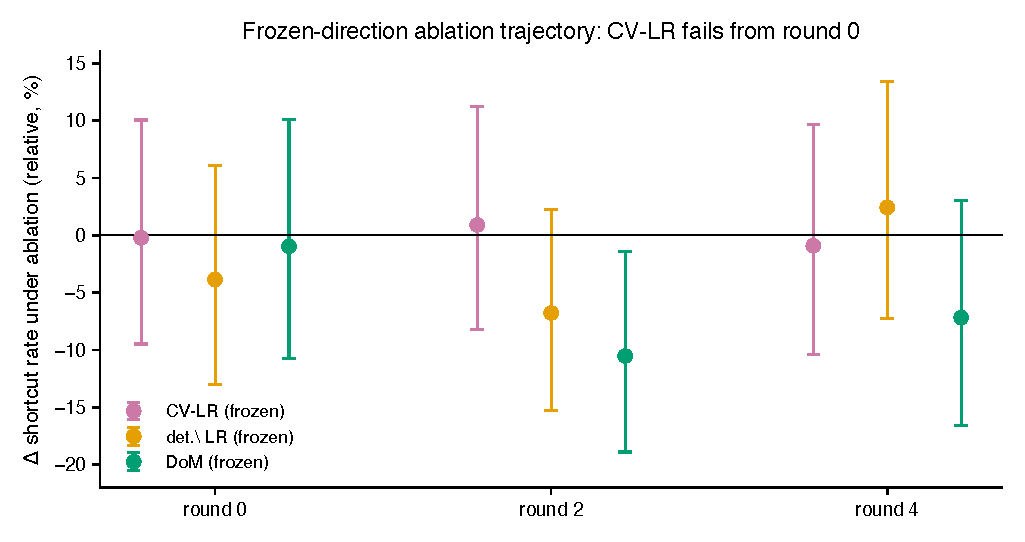
\includegraphics[width=0.75\textwidth]{figures/fig5_ablation_trajectory.pdf}
\caption{\textbf{Frozen-direction ablation across rounds 0, 2, 4.}
CV-LR and deterministic-LR frozen directions produce null ablation
effects at every checkpoint; only DoM excludes zero, and only at
round~2. The dissociation between additive steering (Fig.~\ref{fig:dose})
and projective ablation on the CV-LR frozen direction is present from
the first SFT round, not at a late transition. $n{=}960$ per
condition; binomial-bootstrap 95\% CIs.}
\label{fig:ablation-trajectory}
\end{figure}

\paragraph{Linear methods only.} Non-linear probes (MLPs) and non-linear
steering may behave differently. Our linear setup is a cleaner test
of the linear-direction deployment assumption but does not bound what
non-linear methods can do.

\paragraph{The adversarial follow-up.} Our setting is non-adversarial:
no gradient pressure against the monitor during training. The natural
next experiment adds exactly that: (i) fit a frozen shortcut probe at
base; (ii) during SFT, add a term to the loss that rewards lowering
the probe's score on shortcut completions; (iii) at each checkpoint,
measure both the frozen and a fresh probe's AUROC, and run the full
additive+ablation battery. The prediction falls out of our result: a
frozen probe subjected to direct gradient pressure against its readout
will lose AUROC faster than under non-adversarial SFT, and the
additive--ablation dissociation will appear earlier and larger.
Validating that prediction would convert the present existence proof
into a quantitative monitor-robustness benchmark relevant to AI
control.

% ============================================================================
\section{Conclusion}

The cheapest methodological change that would catch this compound
failure in practice: refit the probe whenever retraining occurs, and
run the projective-ablation test alongside any steering-based
validation before trusting the direction. When directions must be
extracted, difference-of-means retains causal necessity where
logistic regression---even at AUROC 1.0---does not.

The interpretability-for-safety agenda depends on directions being
stable properties of features. Our result shows they are not, under
the mildest form of training pressure---non-adversarial, single-step
SFT. Whether adversarial training pressure accelerates the failure is
the natural and most important follow-up.

\vspace{1em}
\paragraph{Reproducibility.} All experiments use a
SHA-256--fingerprinted CodeContests subset, bfloat16 training and
inference, and a fixed evaluation harness. Code and directional
artifacts are available at the project repository.

% ============================================================================
\bibliographystyle{plainnat}
\bibliography{references}

\end{document}
